\subsubsection{SOLLVE} 

%% {\itshape
%% 
%% 	\begin{enumerate}
%% 	\item Rename this file to your project WBS-projectname.tex, for example 2.3.3.01-XSDK4ECP.tex.
%% 	\item Complete this template for your project.  Limit your text to two pages, not counting citations.  
%% 	\item Please avoid changing the content of main.tex.  
%% 	\item Put any references in a .bib file with the same root name, for example 2.3.3.01-XSDK4ECP.bib.
%% 	\item Remember to include any image files you reference in your text.
%%     \item The files 2.3.3.01-XSDK4ECP.tex, 2.3.3.01-XSDK4ECP.bib and xSDK-diagram.jpeg are included as examples for your reference.  You can remove them from what you upload.
%% 	\end{enumerate}
%% }


\paragraph{Overview}
OpenMP is a directive-based API for intra-node programming that is widely used  in ECP applications. Implementations of OpenMP and  tools to facilitate OpenMP application development.are available in all DOE LCFs.  
The specification is supported by a stable community of vendors, research labs, and academics who
participate in the efforts of the  OpenMP Architecture Review Board (ARB) and its Language Committee to evolve its features.
The mission of the SOLLVE project is to further enhance  OpenMP and its implementations to meet the performance and productivity goals of ECP applications. 

SOLLVE has identified open ECP application software requirements, developed features and/or implementation technology to address them, and created use cases that motivate the need for enhancements. 
 The project continues to identify needs and works to standardize them via 
%In addition to 
active participation in the deliberations of the Language Committee.  
%SOLLVE has moreover produced 
% prototype
%implementations of key new features to support their rapid adoption.

The project is  developing a verification and validation (V\&V) suite to assess implementations and
enable evaluations by DOE  facilities. It is constructing a high-quality,  robust 
OpenMP implementation based on the LLVM compiler. 
%%% BC put in suitable place: resolution of various interoperability 
 SOLLVE plays a critical
role in specifying, implementing, promoting, and deploying functionality
that will enable ECP application developers to reach their goals using OpenMP.
%The project will demonstrate the high impact of new features via their use in selected
%ECP applications.

\paragraph{Key  Challenges}
%\textit{Describe what is hard to do, why it is challenging.}
%need more features, need more implementations (with quality)
Gaps in OpenMP functionality exist as a result of the rapid evolution of node architectures and  base programming languages, as well as a lack of focus on performance portability before version 5.0.  
 Since vendor representatives dominate the  OpenMP Language Committee, effort is needed  to secure their support with regard to the scope of the API, as well as  the syntax and semantics of new features.

%large feature set, many new features are important for ECP
The API has greatly expanded in recent years as some of these gaps are closed, placing a large burden on its implementers. 
The timely provision of  robust implementations of new features that are critical for ECP is therefore particularly challenging.
%%Must we delete this line?
For performance portability, consistent approaches in multiple implementations is highly desirable. Interoperability concerns have emerged as a  new challenge.
 
 %need help to get good performance. 

Given the lack of availability of implementations with features that target accelerators, many existing codes have used alternative APIs for GPUs: a significant effort will be required to replace those approaches by OpenMP. A broad effort is required to develop and apply best practices for new features and platforms. 

\paragraph{Solution Strategy}
We address the challenges by focusing on the following primary activities:

\begin{enumerate}
\item {\bf Application requirements}
Ongoing in-depth interactions with selected ECP application teams have resulted in a list of required extensions, some of which have been met by the recent 5.0 specification.  New needs are being identified. This work informs all other project activities by producing use cases, detailed feedback and example codes. It moreover contributes to the OpenMP Examples document. 
\item {\bf OpenMP specification evolution}
Members of the SOLLVE project are active participants in the OpenMP Language committee.  The project creates early prototypes for new features based on ECP use cases, develops concrete proposals and submits them for standardization. Several proposed features  were included in OpenMP 5.0, ratified November 2018. More are under development for version 5.1.
\item {\bf LLVM  Compiler}
SOLLVE implements new OpenMP features in the LLVM compiler and develops analyses and transformations that enhance, and provide consistency to, OpenMP performance. Its open source solutions may be leveraged in vendor compilers.
The compiler is available on LCF platforms.
\item {\bf Lightweight OpenMP runtime}
The BOLT runtime, built upon ultra-lightweight threading, addresses the need for efficient nested parallelism and improved task scheduling, it develops better support for interoperability with MPI. BOLT is integrated and delivered with the project's LLVM compiler. 
\item {\bf Validation and Verification (V\&V)} 
A V\&V suite is being implemented that allows vendors, users and facilities to assess the coverage
and standard compliance of OpenMP implementations. A ticket system for bug reporting and inquiries has also been deployed to facilitate interaction with end users.
\item{\bf Training and Outreach}
 Tutorials and webinars are delivered to provide information on OpenMP features and their usage, as well as updating on the status of  %their support in vendor and open source 
 implementations. Deeper interaction with application programmers via hackathons supports the development of ECP codes using all available OpenMP features.
%  also provides immediate feedback to compiler and tool developers as the application teams experiment with the use of new features.  
\end{enumerate}
%%revision needed starting here: publications from IWOMP, Lingda, etc.


\paragraph{Recent Progress}
Figure \ref{fig:sollve-update} shows the latest progress on the 5 core SOLLVE
thrust areas. The {\bf training and outreach} activity is a
cross-cutting effort which is supported by resources from SOLLVE and  ECP Broader Engagement,
 with contributions by external collaborators, notably Lawrence Berkeley National
Laboratory.   
%Oak Ridge and Delaware are not external so I commented this out in the hope it can benefit the figure
%project and
%external partners, namely collaborators from Lawrence Berkeley National
%Laboratory, Oak Ridge, University of Delaware and other academic institutions.
A number of articles have also been published
as part of the SOLLVE
effort~\cite{openmp-tr6,zinenko.cc.2018,vandv2019,
tregion, Mishra:2019:KFA:3314872.3314915,
udm, loopTransPragmas, DBLP:conf/iwomp/SreenivasanJHBS19,
DBLP:conf/iwomp/ScoglandSOHES19, DBLP:conf/iwomp/0001WLSS19,
DBLP:conf/iwomp/KaleIKKC19, Bak2019OptimizedEO, lsrt, boltPACT19}.


%% The value that SOLLVE brings to ECP is observed in the ease of leveraging
%% different OpenMP features related to data mappings, parallelism exposure (e.g.
%% {\bf concurrent} or {\bf simd} directives) and control (affinity), runtime
%% scheduling and accelerator (device) offloading (e.g. GPUs or FPGAs).

\begin{figure}[t]
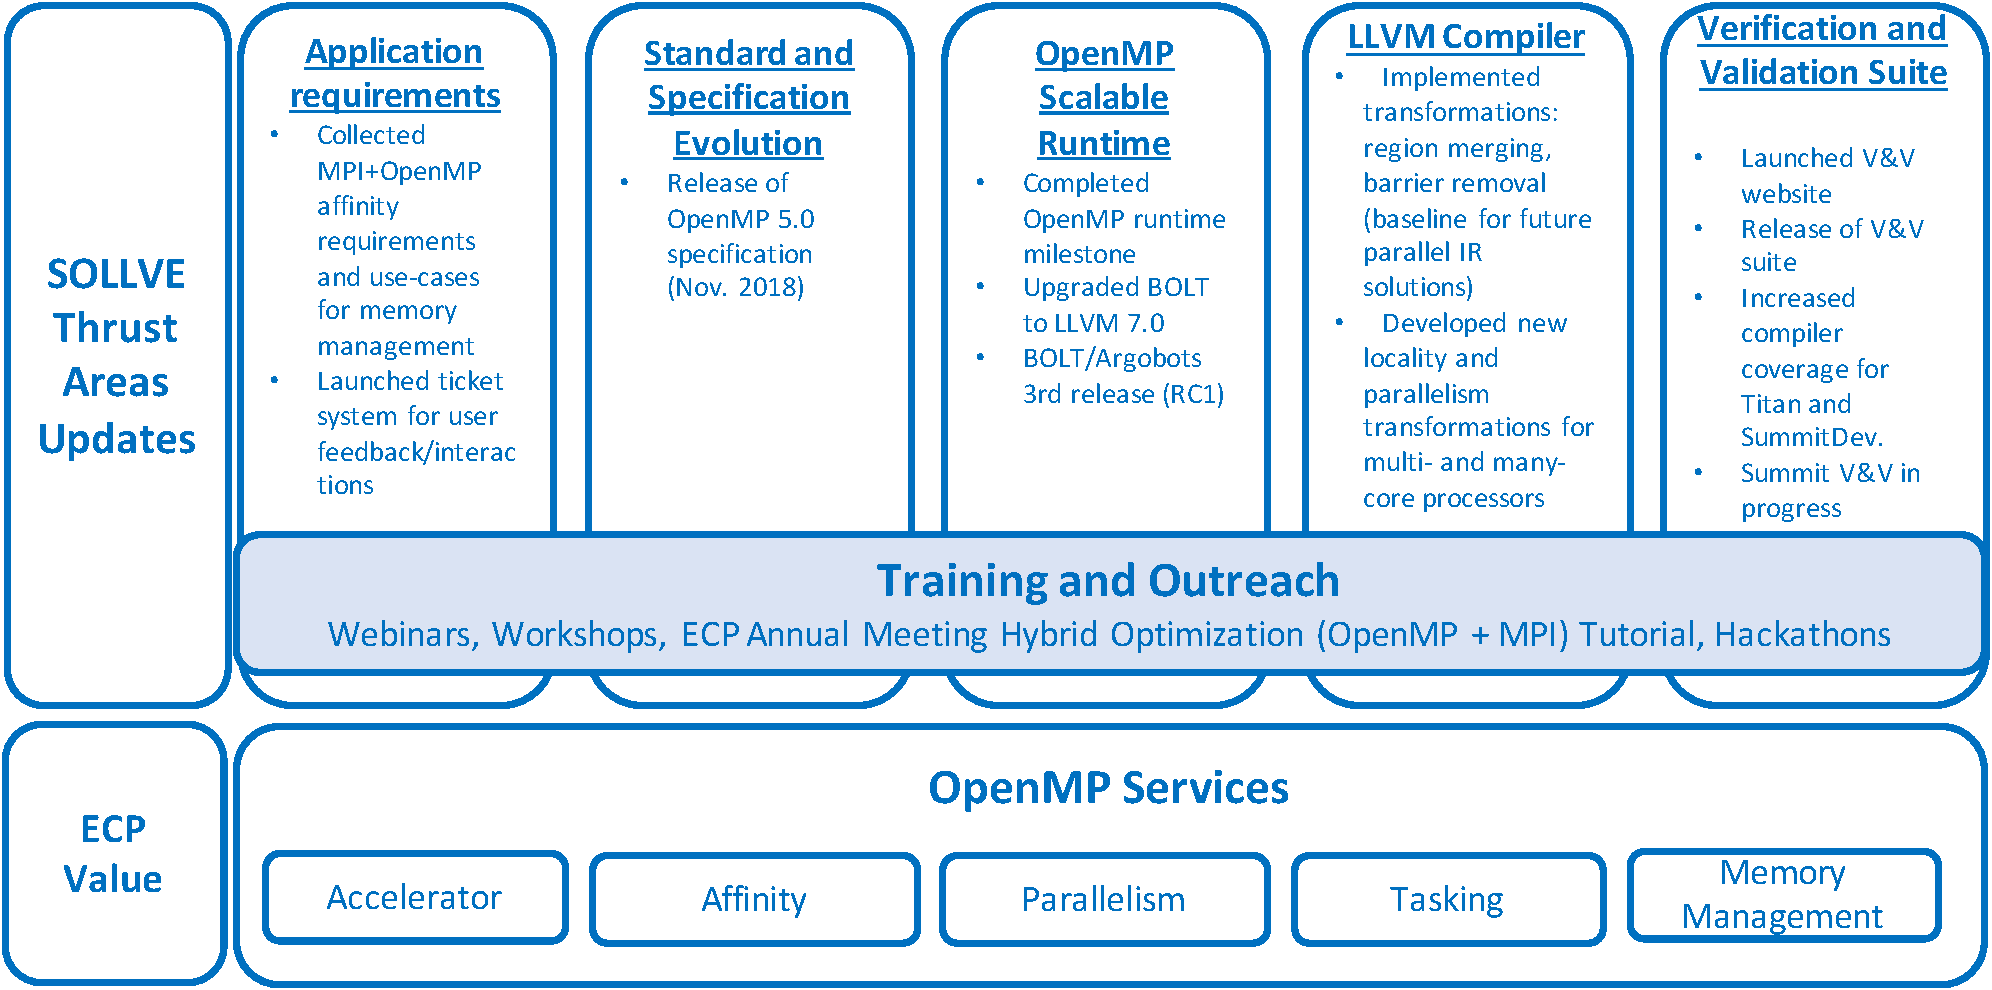
\includegraphics[width=1.0\linewidth,height=9.1cm]{projects/2.3.2-Tools/2.3.2.11-SOLLVE/SOLLVE-progress}
\caption{\label{fig:sollve-update}SOLLVE thrust area updates}
\end{figure}
%\textit{Describe what you have done recently.  It would be good to have some kind of figure or diagram in this section.}

\paragraph{Next Steps}
The following next steps are planned:
\begin{itemize}
\item Applications: Continue to interact with ECP applications teams, evaluate implementations of new features and explore new requirements; 
% create mini-apps to help evaluate OpenMP accelerator support; 
 identify best practices for the use of OpenMP on accelerators;
%for memory management API and concurrent parallel construct; prepare and coordinate %OpenMP webinar focusing on memory management, deep copy and tasking. Spack %package development and deployment with applications. 
\item OpenMP specification: Continue work toward the next version of the standard via ECP-motivated feature development and participation in the OpenMP Language Committee: version 5.1 is already well under way and is due for release November 2020;
%Next face-to-face meeting in January 2019; ratify and vote latest memory management %features and mappers, vote on examples, add to loop scheduling and tasking for affinity %research. 
\item LLVM compiler: Improve performance of device offloading and optimize generation of code within target devices; generalize to enable reuse across multiple offloading architectures; develop infrastructure to support integration of Fortran front end; increase parallel region performance; 
%develop new optimizations for loop transformations; refine Clang based implementation of data layout transformations for OpenMP offloading; improve general testing; evaluate on Summit and other ECP systems. 
\item OpenMP runtime: provide support for 5.0 spec; improve performance of MPI+OpenMP codes; address broader set of interoperability challenges; address advanced tasking requirements;
% and MPI implementations
\item V\&V suite: Continue expanding the coverage of the V\&V Suite, with main focus on 4.5 features;  expand Fortran tests; work with ARB Examples Committee; improve ALCF toolchains;
\end{itemize}

%\textit{Describe what you are working on next.}
